\clearpage
\section*{Task 4 - Point Processing}

\subsection*{Intensity transform}

The gamma correction is done by applying the function $px_{new} = {px_{old}}^{\gamma}$ to every pixel in the image.
Because we're operating with input and output that is integers in the [0, 255] range, not floating point numbers in the [0, 1] range, we need to take this into consideration for the function.
\begin{lstlisting}[language=Python, label=gamma_correction, caption=Gamma correction]
def pixel_wise_transform(matrix, fun):
    return np.asarray(map(lambda row: map(lambda px: fun(px), row), matrix))


def gamma_correct(matrix, gamma=1.0):
    return pixel_wise_transform(matrix, lambda px: int(255 * ((px / 255) ** gamma)))
\end{lstlisting}

For the second part of the task, we need to find the maximum and minimum intensity level of the image.
Using these values, we can again apply a function to every pixel in the image,
which first skews every value towards 0 then scales them so that the largest value becomes 255.

\begin{lstlisting}[language=Python, label=input_range, caption=Input range stretching]
def minmax_2d(matrix):
    return map(lambda f: f(f(matrix, key=lambda x: f(x))), (min, max))


def stretch_range(matrix):
    m_min, m_max = minmax_2d(matrix)
    return pixel_wise_transform(matrix, lambda px: int((px - m_min) / ((m_max - m_min) / 255)))
\end{lstlisting}

\begin{figure}[h!]
    \centering
    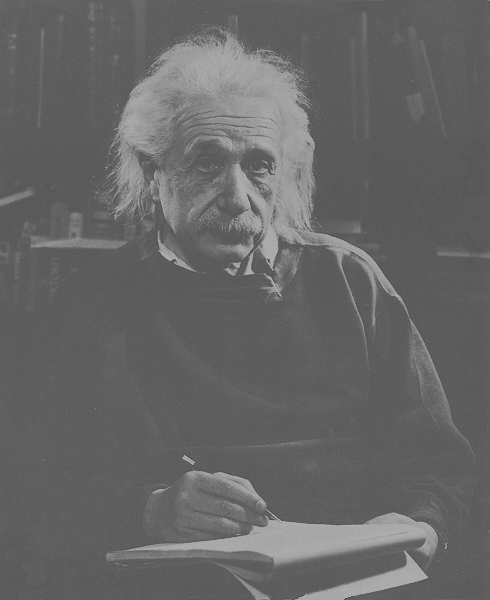
\includegraphics[width=5cm]{../LAB1/img/einstein_lowcontrast.png}
    \includegraphics[width=5cm]{../LAB1/output/gamma_einstein_lowcontrast.png}
    \includegraphics[width=5cm]{../LAB1/output/stretched_gamma_einstein_lowcontrast.png}
    \caption{Left: Original einstein\_lowcontrast.png, middle: gamma corrected, right: input range stretched then gamma corrected.}
\end{figure}

\clearpage
\subsection*{Histogram equalization}

To create a histogram we iterate over the pixels and count the occurrences.
To normalize we need the sum of counts (aka. the picture size), which we divide every count by.
Finally a helper function takes the normalized histogram and returns a cummulative distribution function representing the histogram.

\begin{lstlisting}[language=Python, label=input_range, caption=Input range stretching]
def create_histogram(matrix):
    histogram = defaultdict(int)
    for row in matrix:
        for px in row:
            histogram[px] += 1

    return histogram


def normalize_histogram(histogram):
    normalized = dict()
    total = sum(histogram.values())
    for key, value in histogram.iteritems():
        normalized[key] = value / total

    return normalized


def create_cdf(histo):
    return lambda i: sum(normalized_histogram[j] for j in [v for v in normalized_histogram.keys() if v <= i])
\end{lstlisting}

\begin{figure}[h!]
    \centering
 \begin{verbatim}
 [[2 2 6 6]     [[ 0.25    0.25    0.9375  0.9375]
  [3 3 1 4]      [ 0.375   0.375   0.125   0.6875]
  [0 6 5 4]      [ 0.0625  0.9375  0.75    0.6875]
  [4 4 4 7]]     [ 0.6875  0.6875  0.6875  1.    ]]
 \end{verbatim}
 \caption{Left: Randomly generated matrix. Right: The same matrix after using the cummulative distribution function on every value.}
\end{figure}



